% Course report prepared with the Springer Nature article class, version 3.1
% (December 2024), and a Tribhuvan University project-report front matter.
\documentclass[pdflatex,sn-vancouver-num]{sn-jnl}

\usepackage[T1]{fontenc}
\usepackage{graphicx}
\usepackage{amsmath,amssymb,amsfonts}
\usepackage{newtxtext,newtxmath}
\usepackage{booktabs}
\usepackage{xcolor}
\usepackage{placeins}

\hypersetup{
    pdftitle={Comparative Evaluation of Five Machine Learning Classifiers for Diabetes Outcome Classification},
    pdfauthor={Sandesh Poudel, Sankalpa Gautam, and Tilak Thapa},
    hidelinks
}

\raggedbottom

% Match the project-report convention used in the supplied layout reference.
\renewcommand{\sectionfont}{\normalfont\fontsize{14}{16}\selectfont\bfseries\centering}
\makeatletter
\renewcommand{\ps@plain}{%
    \let\@mkboth\@gobbletwo
    \let\@oddhead\@empty
    \let\@evenhead\@empty
    \def\@oddfoot{\vbox to 18pt{\vfill\reset@font\rmfamily\hfil\thepage\hfil}}%
    \let\@evenfoot\@oddfoot
}
\makeatother

\newcommand{\reportabstract}{This project compares five classifiers for the binary \texttt{Outcome} field in the Pima Indians Diabetes dataset: a custom $k$-nearest neighbours classifier, a decision tree, a calibrated support vector machine, Gaussian Naive Bayes, and a multi-layer perceptron. The 768 records were divided into a stratified training set of 614 records and a held-out test set of 154 records. Following the project's preprocessing rule, zeros in glucose, blood pressure, skin thickness, insulin, and body mass index were treated as missing. Median imputation and standard scaling were fitted on the training set and then applied to the test set. The decision tree achieved the highest accuracy (78.57\%), sensitivity (68.52\%), F1 score (69.16\%), and Matthews correlation coefficient (0.527), while the multi-layer perceptron produced the highest ROC--AUC (81.04\%). The different rankings show that model performance cannot be judged from one measure alone. Since the evaluation used one train--test split of a small and narrowly defined population, the saved pipeline and Streamlit interface are an educational demonstration rather than evidence of clinical performance.}

\newcommand{\reportkeywords}{diabetes classification, machine learning, Pima Indians Diabetes dataset, comparative evaluation, data mining}

\begin{document}

\hypersetup{pageanchor=false}
\begin{titlepage}
\thispagestyle{empty}
\thispdfpagelabel{}
\enlargethispage{4.5cm}
\begin{center}
    \vspace*{0.5cm}
    
\includegraphics[height=3.5cm]{assets/tu-logo.png}

    \vspace{0.35cm}
    {\fontsize{14}{17}\selectfont\bfseries
    TRIBHUVAN UNIVERSITY\par
    INSTITUTE OF ENGINEERING\par
    PURWANCHAL CAMPUS\par}

    \vspace{1.25cm}
    {\fontsize{13}{16}\selectfont\bfseries
    \makebox[\textwidth][c]{DATA WAREHOUSE AND DATA MINING LAB REPORT}\par}

    \vspace{0.35cm}
    {\fontsize{14}{17}\selectfont\bfseries ON\par}

    \vspace{0.35cm}
    {\fontsize{16}{20}\selectfont\bfseries
    \makebox[\textwidth][c]{COMPARATIVE EVALUATION OF FIVE MACHINE}\par
    \makebox[\textwidth][c]{LEARNING CLASSIFIERS FOR DIABETES}\par
    OUTCOME CLASSIFICATION\par}

    \vspace{1.05cm}
    {\fontsize{14}{17}\selectfont\bfseries BY\par}

    \vspace{0.35cm}
    {\fontsize{13}{16}\selectfont\bfseries
    SANDESH POUDEL (PUR079BCT074)\par
    SANKALPA GAUTAM (PUR079BCT078)\par
    TILAK THAPA (PUR079BCT094)\par}

    \vfill
    {\fontsize{12}{15}\selectfont\bfseries
    \makebox[\textwidth][c]{DEPARTMENT OF ELECTRONICS AND COMPUTER ENGINEERING}\par
    PURWANCHAL CAMPUS\par
    DHARAN, NEPAL\par}

    \vspace{0.75cm}
    {\fontsize{13}{16}\selectfont\bfseries AUGUST 2026\par}
\end{center}
\end{titlepage}
\hypersetup{pageanchor=true}

\pagenumbering{roman}
\setcounter{page}{1}
\pagestyle{plain}

\section*{ABSTRACT}
\phantomsection
\addcontentsline{toc}{section}{ABSTRACT}
\noindent\reportabstract\par
\vspace{0.5cm}
\noindent\textbf{Keywords:} \reportkeywords\par

\clearpage
\renewcommand{\contentsname}{TABLE OF CONTENTS}
\pdfbookmark[1]{TABLE OF CONTENTS}{table-of-contents}
\tableofcontents

\clearpage
\phantomsection
\addcontentsline{toc}{section}{LIST OF ABBREVIATIONS}
\section*{LIST OF ABBREVIATIONS}
\vspace{0.5cm}
\begin{center}
\renewcommand{\arraystretch}{1.25}
\begin{tabular}{@{}p{0.19\textwidth}p{0.67\textwidth}@{}}
AUC & Area under the curve \\
BMI & Body mass index \\
CSV & Comma-separated values \\
FN & False negative \\
FP & False positive \\
KNN & $k$-nearest neighbours \\
MCC & Matthews correlation coefficient \\
MLP & Multi-layer perceptron \\
RBF & Radial basis function \\
ReLU & Rectified linear unit \\
ROC & Receiver operating characteristic \\
SVM & Support vector machine \\
TN & True negative \\
TP & True positive \\
\end{tabular}
\end{center}

\clearpage
\pagenumbering{arabic}
\setcounter{page}{1}

\section{INTRODUCTION}\label{sec:introduction}

Diabetes is a chronic metabolic disease characterized by elevated blood glucose. Without appropriate management, it can damage the heart, blood vessels, eyes, kidneys, and nerves \cite{who2024diabetes}. This project does not attempt to make a clinical diagnosis. It asks a controlled laboratory question: how do five familiar classifiers compare when they use the same data split and preprocessing pipeline?

The models are a custom implementation of $k$-nearest neighbours (KNN), a decision tree, a calibrated support vector machine (SVM), Gaussian Naive Bayes, and a multi-layer perceptron (MLP). They are evaluated using accuracy, precision, sensitivity, specificity, F1 score, receiver operating characteristic area under the curve (ROC--AUC), and Matthews correlation coefficient (MCC). Multiple measures are needed because the two outcome classes are unequal and the models make different kinds of errors.

Zeros in five physiological measurements are handled as missing values under the project's preprocessing rule. The imputation and scaling parameters are learned from the training data only, preventing test records from influencing model fitting. The repository reproduces the audit, preprocessing, model fitting, evaluation, tables, and figures reported here. It also contains the NumPy implementation of KNN and the Streamlit interface built around the saved MLP pipeline.

\section{RELATED WORK}\label{sec:related}

The CSV analyzed in this project was obtained from the Pima Indians Diabetes Database hosted on Kaggle by UCI Machine Learning \cite{uciKagglePima}. The repository's original README records that address, and the current CSV is byte-for-byte identical to the file stored in the first commit. Kaggle attributes the data to the National Institute of Diabetes and Digestive and Kidney Diseases and cites the earlier study by Smith et al. \cite{uciKagglePima}. Smith and colleagues described the clinical variables and used them to study the onset of diabetes in a high-risk Pima population \cite{smith1988adap}.

The five model families in this report also have different foundations. Nearest-neighbour classification assigns a label from nearby training examples \cite{cover1967nearest}. Classification trees divide the feature space with a sequence of learned rules \cite{breiman1984cart}. Support-vector machines seek a separating boundary with a large margin and can use kernels for non-linear patterns \cite{cortes1995svm}. Neural networks learn layered representations through weight updates such as back-propagation \cite{rumelhart1986backprop}. For this project, all five were therefore run with the same split and preprocessing instead of treating model complexity as a guarantee of better performance.

\section{MATERIALS AND METHODS}\label{sec:methods}

\subsection{Experimental workflow}\label{subsec:workflow}

Figure~\ref{fig:workflow} summarizes the full experiment. The raw data were audited before a stratified split was made. The imputer and scaler were then fitted on the training portion only. All five classifiers received the same transformed features, and evaluation took place once on the untouched test set. Finally, the fitted preprocessing steps and MLP were stored as one pipeline for the demonstration app.

\begin{figure}[t]
    \centering
    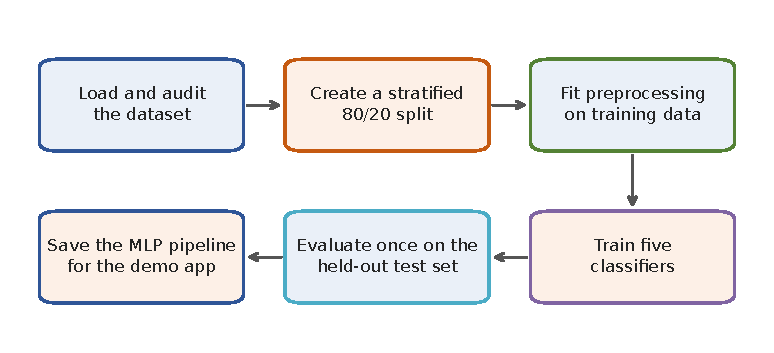
\includegraphics[width=\textwidth]{figures/workflow.pdf}
    \caption{Experimental workflow from data audit and preprocessing to evaluation and creation of the application pipeline.}
    \label{fig:workflow}
\end{figure}

\subsection{Dataset description}\label{subsec:dataset}

The local dataset contains 768 rows, eight predictors, and one target column named \texttt{Outcome}. Outcome 0 appears in 500 records (65.10\%), and outcome 1 appears in 268 records (34.90\%). No fully duplicated rows were found. The variables are listed in Table~\ref{tab:variables}; their descriptions follow the Kaggle data card and the original study \cite{uciKagglePima,smith1988adap}.

\begin{table}[t]
\caption{Variables in the local Pima Indians Diabetes dataset.}\label{tab:variables}
\centering
\begin{tabular}{@{}p{0.31\textwidth}p{0.61\textwidth}@{}}
\toprule
Variable & Meaning \\
\midrule
Pregnancies & Number of recorded pregnancies \\
Glucose & Plasma glucose concentration after a two-hour oral glucose tolerance test (mg/dL) \\
BloodPressure & Diastolic blood pressure (mmHg) \\
SkinThickness & Triceps skin-fold thickness (mm) \\
Insulin & Two-hour serum insulin ($\mu$U/mL) \\
BMI & Body mass index ($\mathrm{kg}/\mathrm{m}^{2}$) \\
DiabetesPedigreeFunction & Dataset-specific score summarizing family history \\
Age & Age in years \\
Outcome & Recorded class: 0 (no diabetes) or 1 (diabetes) \\
\bottomrule
\end{tabular}
\end{table}

The Kaggle data card states that every record is from a woman of Pima Indian heritage who was at least 21 years old \cite{uciKagglePima}. The sample therefore does not represent the general population. Throughout this report, ``diabetes'' means the class recorded in \texttt{Outcome}; it is not a diagnosis made by the software.

\subsection{Data audit and preprocessing}\label{subsec:preprocessing}

Under the preprocessing rule chosen for this experiment, zeros in five measurement columns represent missing observations. Figure~\ref{fig:audit} shows both the class distribution and the number of affected rows. Insulin has the largest number (374), followed by skin thickness (227). The counts for blood pressure, BMI, and glucose are 35, 11, and 5 respectively. Zeros in pregnancies and age were not changed because those columns were not included in this rule.

\begin{figure}[t]
    \centering
    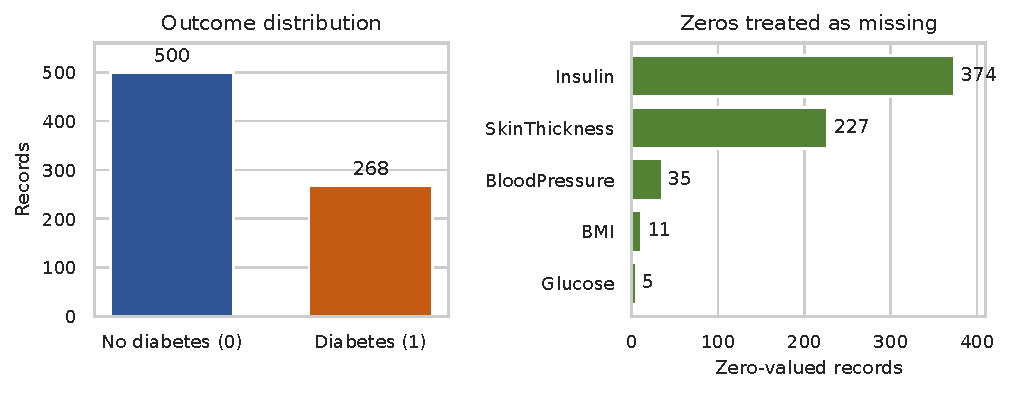
\includegraphics[width=\textwidth]{figures/dataset_audit.pdf}
    \caption{Class distribution and zero counts in the five physiological measurements treated as missing.}
    \label{fig:audit}
\end{figure}

The data were separated before any imputation or scaling. A stratified 80/20 split with \texttt{random\_state=42} produced 614 training rows and 154 test rows. The training set contains 400 negative and 214 positive examples; the test set contains 100 negative and 54 positive examples.

Within the training data, zero values in the five selected columns were replaced by each column's non-zero median. The learned medians were 117 for glucose, 72 for blood pressure, 29 for skin thickness, 125 for insulin, and 32.4 for BMI. The same fixed medians were then applied to the test data. Standard scaling was fitted after imputation, again using training data only. For feature $x_j$, the transformation was

\begin{equation}
z_j = \frac{x_j-\mu_j}{\sigma_j},
\label{eq:standardization}
\end{equation}

where $\mu_j$ and $\sigma_j$ are the mean and standard deviation learned from the training set. Scikit-learn pipelines and column transformations were used to keep these operations together \cite{pedregosa2011scikit}. This arrangement also ensures that the app applies the same transformation used during training.

For the correlation heatmap, zeros in the same five features were changed to missing values and Pearson correlations were calculated from the available pairs. This descriptive calculation was separate from the model-training pipeline.

\subsection{Software and reproducibility}\label{subsec:software}

The experiment was run with Python 3.12, scikit-learn 1.9.0, pandas 2.3.3, NumPy 2.5.2, Matplotlib 3.11.1, and seaborn 0.13.2. KNN was implemented directly with NumPy; the other models and evaluation measures use scikit-learn \cite{pedregosa2011scikit}. The run used an x86-64 computer with a 13th-generation Intel Core i7-13620H processor and 31 GiB of memory, without GPU acceleration.

The repository pins its dependencies and records the random seed and model settings. Running \texttt{generate\_figures.py} repeats the experiment and recreates the numerical results, tables, and figures used in this report. The build also checks that these outputs agree with the values quoted in the manuscript.

\section{MACHINE LEARNING CLASSIFIERS}\label{sec:models}

Table~\ref{tab:settings} lists the fixed settings used for each classifier. The experiment did not include a grid search or repeated hyperparameter tuning.

\begin{table}[!htbp]
\caption{Classifier settings used in the experiment.}\label{tab:settings}
\centering
\begin{tabular}{@{}p{0.25\textwidth}p{0.67\textwidth}@{}}
\toprule
Classifier & Main settings \\
\midrule
Custom KNN & $k=7$; Euclidean distance; uniform majority vote \\
Decision Tree & Gini criterion; maximum depth 4; minimum split size 10; seed 42 \\
Calibrated SVM & RBF kernel; $C=1$; $\gamma=\texttt{scale}$; five-fold sigmoid calibration; \texttt{ensemble=False} \\
Gaussian Naive Bayes & Scikit-learn default variance smoothing \\
MLP & Hidden layers (16, 8); ReLU; Adam; $\alpha=0.01$; at most 1000 iterations; seed 42 \\
\bottomrule
\end{tabular}
\end{table}

\subsection{Custom \texorpdfstring{$k$}{k}-nearest neighbours}\label{subsec:knn}

KNN stores the training examples and compares a new row with them. For two standardized feature vectors $\mathbf{x}$ and $\mathbf{x}_i$, the Euclidean distance is

\begin{equation}
d(\mathbf{x},\mathbf{x}_i)=\sqrt{\sum_{j=1}^{8}(x_j-x_{ij})^2}.
\label{eq:distance}
\end{equation}

The implementation selects the seven smallest distances and predicts the majority class. Its score for class 1 is the fraction of these seven neighbours that belong to class 1. Scaling matters for KNN because otherwise a large-range feature can dominate the distance. The general nearest-neighbour principle is described by Cover and Hart \cite{cover1967nearest}.

\subsection{Decision tree}\label{subsec:tree}

The decision tree recursively divides rows using one feature at a time. Candidate splits were evaluated with Gini impurity,

\begin{equation}
G = 1-\sum_{c\in\{0,1\}}p_c^2,
\label{eq:gini}
\end{equation}

where $p_c$ is the class proportion in a node. Maximum depth 4 and minimum split size 10 limit the tree's complexity. These settings were intended to reduce overfitting. The approach follows the classification-tree family described by Breiman et al. \cite{breiman1984cart}.

\subsection{Calibrated support vector machine}\label{subsec:svm}

The SVM used a radial basis function kernel,

\begin{equation}
K(\mathbf{x},\mathbf{x}')=\exp\left(-\gamma\lVert\mathbf{x}-\mathbf{x}'\rVert^2\right),
\label{eq:rbf}
\end{equation}

with $C=1$ and scikit-learn's scaled value of $\gamma$. The kernel lets the classifier form a non-linear boundary in the transformed feature space. SVMs originate from the maximum-margin method developed by Cortes and Vapnik \cite{cortes1995svm}. Five-fold sigmoid calibration produced the scores used to construct the ROC curve. Calibration error was not evaluated separately.

\subsection{Gaussian Naive Bayes}\label{subsec:nb}

Gaussian Naive Bayes models each feature as normally distributed within each class and combines the feature likelihoods using Bayes' rule. Its main simplification is conditional independence between features after the class is known. That assumption is unlikely to be exact for clinical measurements, but the model remains a useful lightweight baseline. The implementation used the default scikit-learn settings \cite{pedregosa2011scikit}.

\subsection{Multi-layer perceptron}\label{subsec:mlp}

The MLP contains two hidden layers with 16 and 8 units. Rectified linear unit activation was used in each hidden layer, and the Adam optimizer updated the weights. The regularization value $\alpha=0.01$ penalizes large weights. Training was allowed to continue for at most 1000 iterations with seed 42. The model follows the layered learning and back-propagation idea described by Rumelhart et al. \cite{rumelhart1986backprop}.

The MLP, imputer, and scaler were saved together in one joblib pipeline. The Streamlit interface accepts the same eight inputs and applies the fitted preprocessing steps before displaying the model's predicted class and score. The interface labels the output as a model estimate rather than medical advice.

\section{EVALUATION METRICS}\label{sec:metrics}

Let true positives (TP) and true negatives (TN) be correctly classified positive and negative rows. False positives (FP) are negative rows classified as positive, and false negatives (FN) are positive rows classified as negative. The threshold-based measures are

\begin{align}
\text{Accuracy} &= \frac{TP+TN}{TP+TN+FP+FN}, \label{eq:accuracy}\\
\text{Precision} &= \frac{TP}{TP+FP}, \label{eq:precision}\\
\text{Sensitivity} &= \frac{TP}{TP+FN}, \label{eq:sensitivity}\\
\text{Specificity} &= \frac{TN}{TN+FP}, \label{eq:specificity}\\
F_1 &= \frac{2\,\text{Precision}\,\text{Sensitivity}}
{\text{Precision}+\text{Sensitivity}}. \label{eq:f1}
\end{align}

Accuracy gives the overall correct fraction. Precision describes how many positive predictions are correct, while sensitivity describes how many recorded positives are found. Specificity measures how many negatives are correctly rejected. F1 is the harmonic mean of precision and sensitivity.

MCC uses all four confusion-matrix counts:

\begin{equation}
\mathrm{MCC}=\frac{TP\times TN-FP\times FN}
{\sqrt{(TP+FP)(TP+FN)(TN+FP)(TN+FN)}}.
\label{eq:mcc}
\end{equation}

MCC was introduced by Matthews \cite{matthews1975mcc} and is useful when class counts are unequal because a high value requires agreement in both classes \cite{chicco2020mcc}. Its range is $-1$ to 1, where 1 indicates perfect agreement, 0 is no better than uncorrelated predictions, and $-1$ indicates complete disagreement.

ROC curves show sensitivity against false-positive rate over many score thresholds \cite{fawcett2006roc}. ROC--AUC summarizes this curve and can be interpreted as the probability that a randomly selected positive row receives a higher score than a randomly selected negative row \cite{hanley1982auc}. A value of 0.5 corresponds to chance ranking and 1 indicates perfect ranking. AUC does not select a clinical decision threshold and does not prove that the scores are well calibrated.

\section{RESULTS AND DISCUSSION}\label{sec:results}

\subsection{Exploratory observations}\label{subsec:eda}

The class audit in Figure~\ref{fig:audit} shows a moderate imbalance toward outcome 0. A classifier that always predicts 0 would therefore obtain 65.10\% accuracy while failing to identify any positive row. This is why the evaluation includes sensitivity, F1, AUC, and MCC rather than accuracy alone.

Figure~\ref{fig:correlation} presents pairwise Pearson correlations after treating the selected zeros as missing for this descriptive calculation. Glucose has the largest linear relationship with Outcome ($r=0.49$), followed by BMI ($r=0.31$), insulin ($r=0.30$), skin thickness ($r=0.26$), and age ($r=0.24$). These correlations describe linear relationships in this sample and do not imply causation.

\begin{figure}[t]
    \centering
    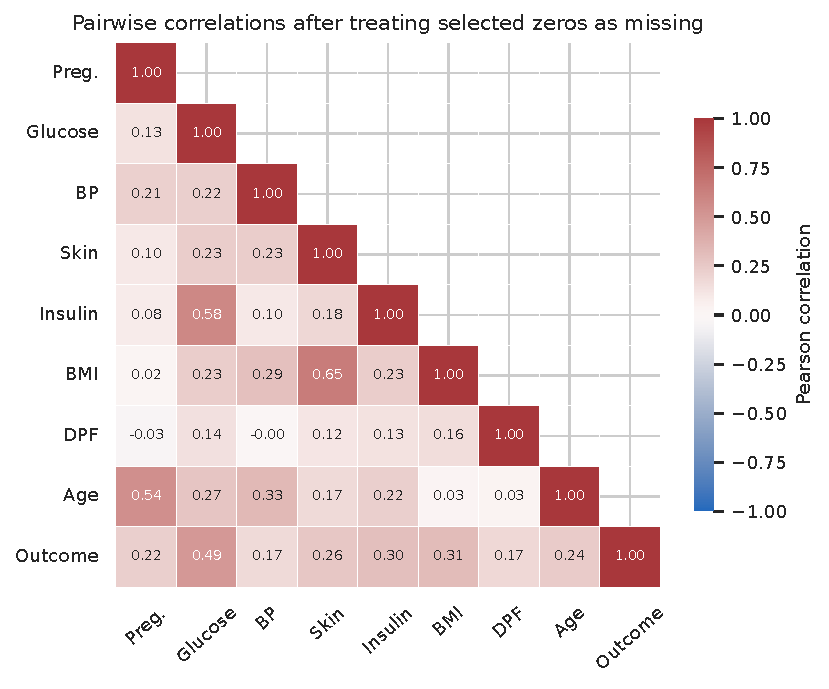
\includegraphics[width=0.88\textwidth]{figures/correlation_heatmap.pdf}
    \caption{Lower-triangle Pearson correlation matrix. Selected zeros in the five measurement fields were treated as missing and omitted pairwise.}
    \label{fig:correlation}
\end{figure}

\subsection{Model comparison}\label{subsec:comparison}

Table~\ref{tab:metrics} gives the complete held-out results. The decision tree produced the highest accuracy (78.57\%), precision (69.81\%), sensitivity (68.52\%), F1 (69.16\%), and MCC (0.527). It also shared the highest specificity (84.00\%) with the calibrated SVM. The MLP had the highest ROC--AUC (81.04\%).

\begin{table}[!htbp]
\caption{Performance on the 154-row held-out test set. Percentage values are shown except for MCC. Bold marks the best value in each column; the specificity maximum is tied.}\label{tab:metrics}
\centering
\footnotesize
\setlength{\tabcolsep}{2.5pt}
\input{generated/model_metrics.tex}
\end{table}

\begin{figure}[t]
    \centering
    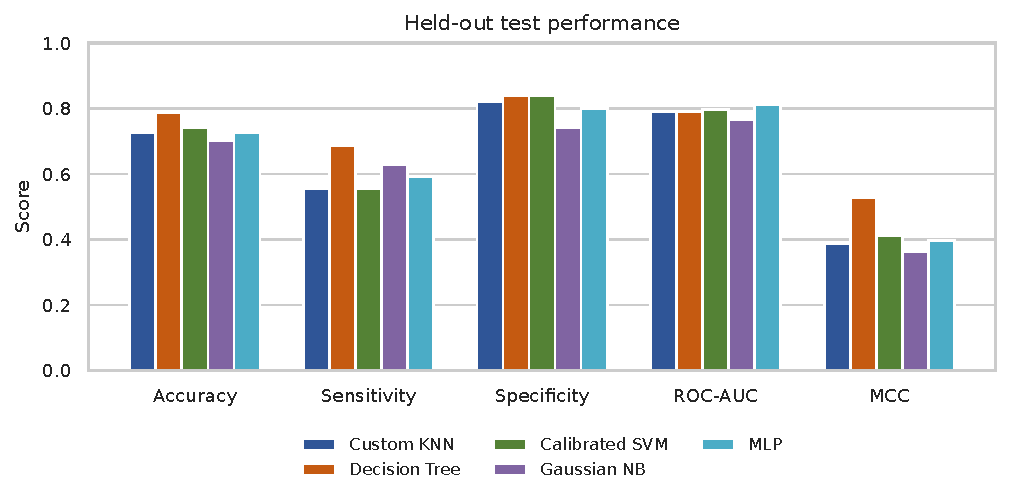
\includegraphics[width=\textwidth]{figures/model_comparison.pdf}
    \caption{Test performance of the five classifiers across the selected evaluation measures.}
    \label{fig:comparison}
\end{figure}

Model choice depends on the evaluation measure. At the default classification threshold, the decision tree produced the strongest threshold-based results, while the MLP produced the highest AUC across thresholds. The MLP's AUC exceeded that of the calibrated SVM by only 1.41 percentage points. Since the experiment used one split without a significance test or repeated cross-validation, this difference is an observed result rather than proof of superiority.

\subsection{Error patterns}\label{subsec:errors}

Figure~\ref{fig:confusion} shows the confusion matrix for each model. The decision tree correctly classified 84 of 100 negative rows and 37 of 54 positive rows. It made 16 false-positive and 17 false-negative errors. KNN and the calibrated SVM each found only 30 positive rows and missed 24. Gaussian Naive Bayes found 34 positives but produced 26 false positives, which explains its higher sensitivity than KNN and SVM but lower specificity. The MLP was between these cases, with 32 true positives, 22 false negatives, 80 true negatives, and 20 false positives.

\begin{figure}[t]
    \centering
    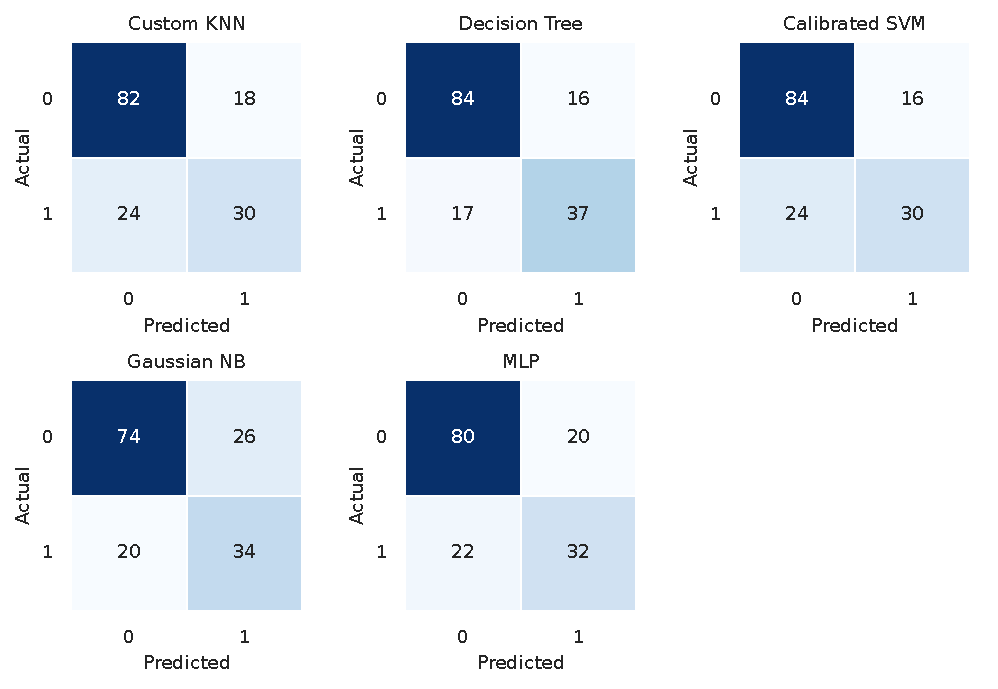
\includegraphics[width=\textwidth]{figures/confusion_matrices.pdf}
    \caption{Confusion matrices for the held-out test set. Rows are actual labels and columns are predicted labels.}
    \label{fig:confusion}
\end{figure}

False negatives and false positives may carry different costs in practice. This experiment did not define those costs or select a clinical operating threshold, so the confusion matrices are used only to compare model error patterns.

\subsection{ROC analysis}\label{subsec:roc}

The ROC curves in Figure~\ref{fig:roc} are all above the chance diagonal for most thresholds. MLP has the largest measured area, followed by the calibrated SVM, KNN, decision tree, and Gaussian Naive Bayes. The ordering differs from accuracy because AUC considers score ranking across thresholds, while accuracy uses one set of predicted labels.

\begin{figure}[t]
    \centering
    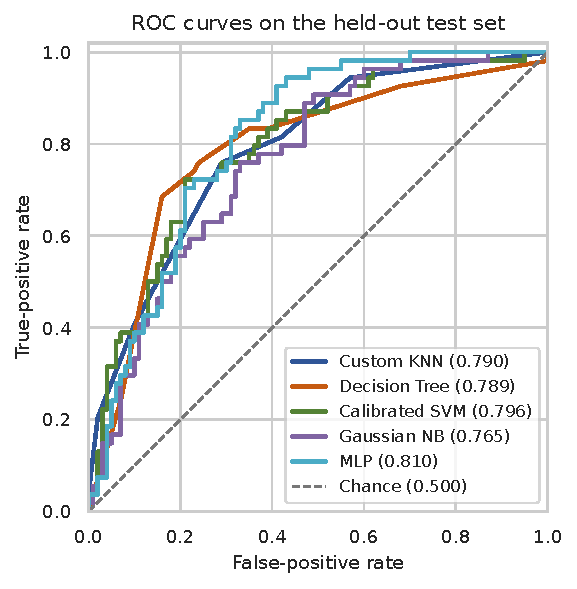
\includegraphics[width=0.84\textwidth]{figures/roc_curves.pdf}
    \caption{ROC curves and AUC values on the held-out test set. The diagonal line represents chance-level ranking.}
    \label{fig:roc}
\end{figure}

\subsection{Exploratory feature sensitivity}\label{subsec:importance}

Permutation importance was calculated for the fitted MLP pipeline from the reproducible report run by shuffling one raw test feature at a time, repeating the shuffle 30 times, and measuring the change in ROC--AUC. On this test set, glucose produced the largest mean decrease (0.117), followed by age (0.053). BMI and insulin had smaller positive values, while blood pressure and skin thickness were close to zero.

\begin{figure}[!htbp]
    \centering
    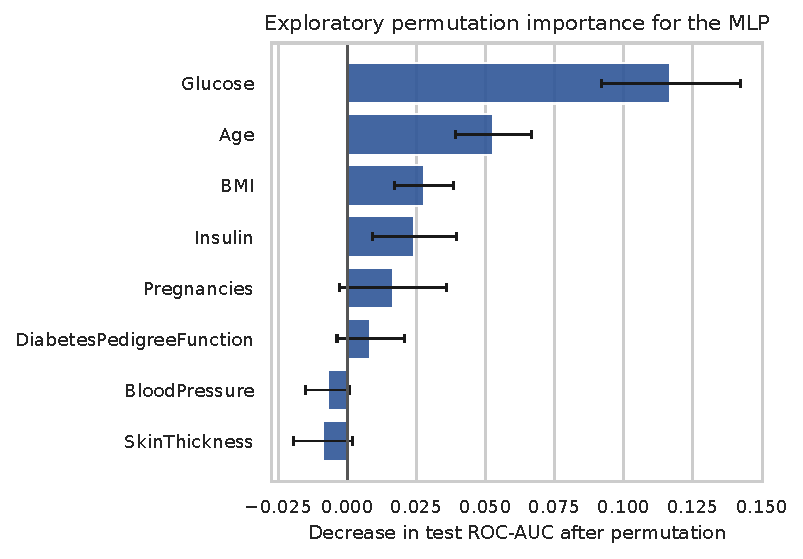
\includegraphics[width=0.88\textwidth]{figures/permutation_importance.pdf}
    \caption{Exploratory MLP permutation importance based on 30 shuffles per feature. Error bars show one standard deviation across shuffles. Negative values can occur from sampling variation.}
    \label{fig:importance}
\end{figure}

Permutation importance is descriptive rather than causal. Correlated predictors may divide importance between them, and estimates based on 154 test records can vary substantially. These values were not used to tune the model.

\subsection{Deployment demonstration}\label{subsec:deployment}

The Streamlit application uses the MLP pipeline stored at \path{out/models/diabetes_pipeline.joblib} because the MLP achieved the highest AUC in the comparison. Keeping the imputer, scaler, column order, and model in one artifact ensures that the application applies the same preprocessing used during training.

The MLP was selected after the test results were examined, so the application does not provide an independent validation result. Its score is not an externally calibrated estimate of patient risk, and the interface is not suitable for diagnosis, screening, or treatment decisions.

\subsection{Limitations}\label{subsec:limitations}

The experiment has several important limitations:

\begin{itemize}
    \item The dataset is small and restricted to women aged 21 years or older of Pima Indian heritage. Performance may differ in other populations.
    \item Evaluation used one stratified train--test split. Repeated validation, uncertainty intervals, and external test data were not included.
    \item The classifiers used fixed settings without a documented hyperparameter search. The MLP was also selected for the application after the test results were known.
    \item The code treats zeros as missing in five measurements. The Kaggle data card does not explain those zero values, so this is a modelling decision rather than a verified property of every record. Median replacement can also hide patterns in missingness without recovering the original measurements.
    \item The positive class is smaller, and the experiment did not use class weighting or threshold optimization.
    \item Clinical calibration, subgroup analysis, prospective testing, and external validation were outside the scope of this project.
\end{itemize}

\FloatBarrier
\section{CONCLUSION}\label{sec:conclusion}

This project compared five classifiers using one consistent, training-only preprocessing workflow. On the held-out test set, the decision tree gave the highest accuracy, sensitivity, F1, and MCC, while the MLP gave the highest ROC--AUC. The difference in rankings shows why a model should not be selected from accuracy alone. Confusion matrices were also necessary to see the balance between missed positives and false alarms.

The project produced a reproducible comparison of five classifiers and connected the saved MLP pipeline to a working Streamlit interface. The results describe this dataset and fixed split only; they do not establish a clinically valid diabetes predictor. The application should therefore be understood as an educational demonstration of the completed machine learning workflow.

\backmatter

\clearpage
\phantomsection
\addcontentsline{toc}{section}{REFERENCES}
\bibliography{references}

\end{document}
